%!TEX program = xelatex+makeindex+bibtex
\documentclass[final]{scrreprt} %scrreprt of scrartcl
% Include all project wide packages here.
\usepackage{fullpage}
\usepackage{polyglossia}
\setmainlanguage{english}
\usepackage{csquotes}
\usepackage{graphicx}
\usepackage{epstopdf}
\usepackage{pdfpages}
\usepackage{caption}
\usepackage[list=true]{subcaption}
\usepackage{float}
\usepackage{standalone}
\usepackage{import}
\usepackage{tocloft}
\usepackage{wrapfig}
\usepackage{authblk}
\usepackage{array}
\usepackage{booktabs}
\usepackage[toc,page,title,titletoc]{appendix}
\usepackage{xunicode}
\usepackage{fontspec}
\usepackage{pgfplots}
\usepackage{SIunits}
\usepackage{units}
\pgfplotsset{compat=newest}
\pgfplotsset{plot coordinates/math parser=false}
\newlength\figureheight 
\newlength\figurewidth
\usepackage{amsmath}
\usepackage{mathtools}
\usepackage{unicode-math}
\usepackage[
    backend=bibtexu,
	texencoding=utf8,
bibencoding=utf8,
    style=ieee,
    sortlocale=en_US,
    language=auto
]{biblatex}
\usepackage{listings}
\newcommand{\includecode}[3][c]{\lstinputlisting[caption=#2, escapechar=, style=#1]{#3}}
\newcommand{\superscript}[1]{\ensuremath{^{\textrm{#1}}}}
\newcommand{\subscript}[1]{\ensuremath{_{\textrm{#1}}}}


\newcommand{\chapternumber}{\thechapter}
\renewcommand{\appendixname}{Bijlage}
\renewcommand{\appendixtocname}{Bijlagen}
\renewcommand{\appendixpagename}{Bijlagen}

\usepackage[hidelinks]{hyperref} %<--------ALTIJD ALS LAATSTE

\renewcommand{\familydefault}{\sfdefault}

\setmainfont[Ligatures=TeX]{Myriad Pro}
\setmathfont{Asana Math}
\setmonofont{Lucida Console}

\usepackage{titlesec, blindtext, color}
\definecolor{gray75}{gray}{0.75}
\newcommand{\hsp}{\hspace{20pt}}
\titleformat{\chapter}[hang]{\Huge\bfseries}{\chapternumber\hsp\textcolor{gray75}{|}\hsp}{0pt}{\Huge\bfseries}
\renewcommand{\familydefault}{\sfdefault}
\renewcommand{\arraystretch}{1.2}
\setlength\parindent{0pt}

%For code listings
\definecolor{black}{rgb}{0,0,0}
\definecolor{browntags}{rgb}{0.65,0.1,0.1}
\definecolor{bluestrings}{rgb}{0,0,1}
\definecolor{graycomments}{rgb}{0.4,0.4,0.4}
\definecolor{redkeywords}{rgb}{1,0,0}
\definecolor{bluekeywords}{rgb}{0.13,0.13,0.8}
\definecolor{greencomments}{rgb}{0,0.5,0}
\definecolor{redstrings}{rgb}{0.9,0,0}
\definecolor{purpleidentifiers}{rgb}{0.01,0,0.01}


\lstdefinestyle{csharp}{
language=[Sharp]C,
showspaces=false,
showtabs=false,
breaklines=true,
showstringspaces=false,
breakatwhitespace=true,
escapeinside={(*@}{@*)},
columns=fullflexible,
commentstyle=\color{greencomments},
keywordstyle=\color{bluekeywords}\bfseries,
stringstyle=\color{redstrings},
identifierstyle=\color{purpleidentifiers},
basicstyle=\ttfamily\small}

\lstdefinestyle{c}{
language=C,
showspaces=false,
showtabs=false,
breaklines=true,
showstringspaces=false,
breakatwhitespace=true,
escapeinside={(*@}{@*)},
columns=fullflexible,
commentstyle=\color{greencomments},
keywordstyle=\color{bluekeywords}\bfseries,
stringstyle=\color{redstrings},
identifierstyle=\color{purpleidentifiers},
}

\lstdefinestyle{matlab}{
language=Matlab,
showspaces=false,
showtabs=false,
breaklines=true,
showstringspaces=false,
breakatwhitespace=true,
escapeinside={(*@}{@*)},
columns=fullflexible,
commentstyle=\color{greencomments},
keywordstyle=\color{bluekeywords}\bfseries,
stringstyle=\color{redstrings},
identifierstyle=\color{purpleidentifiers}
}

\lstdefinestyle{vhdl}{
language=VHDL,
showspaces=false,
showtabs=false,
breaklines=true,
showstringspaces=false,
breakatwhitespace=true,
escapeinside={(*@}{@*)},
columns=fullflexible,
commentstyle=\color{greencomments},
keywordstyle=\color{bluekeywords}\bfseries,
stringstyle=\color{redstrings},
identifierstyle=\color{purpleidentifiers}
}

\lstdefinestyle{xaml}{
language=XML,
showspaces=false,
showtabs=false,
breaklines=true,
showstringspaces=false,
breakatwhitespace=true,
escapeinside={(*@}{@*)},
columns=fullflexible,
commentstyle=\color{greencomments},
keywordstyle=\color{redkeywords},
stringstyle=\color{bluestrings},
tagstyle=\color{browntags},
morestring=[b]",
  morecomment=[s]{<?}{?>},
  morekeywords={xmlns,version,typex:AsyncRecords,x:Arguments,x:Boolean,x:Byte,x:Char,x:Class,x:ClassAttributes,x:ClassModifier,x:Code,x:ConnectionId,x:Decimal,x:Double,x:FactoryMethod,x:FieldModifier,x:Int16,x:Int32,x:Int64,x:Key,x:Members,x:Name,x:Object,x:Property,x:Shared,x:Single,x:String,x:Subclass,x:SynchronousMode,x:TimeSpan,x:TypeArguments,x:Uid,x:Uri,x:XData,Grid.Column,Grid.ColumnSpan,Click,ClipToBounds,Content,DropDownOpened,FontSize,Foreground,Header,Height,HorizontalAlignment,HorizontalContentAlignment,IsCancel,IsDefault,IsEnabled,IsSelected,Margin,MinHeight,MinWidth,Padding,SnapsToDevicePixels,Target,TextWrapping,Title,VerticalAlignment,VerticalContentAlignment,Width,WindowStartupLocation,Binding,Mode,OneWay,xmlns:x}
}

%defaults
\lstset{
basicstyle=\ttfamily\small,
extendedchars=false,
numbers=left,
numberstyle=\ttfamily\tiny,
stepnumber=1,
tabsize=4,
numbersep=5pt
}
\addbibresource{../../library/bibliography.bib}
\begin{document}

\chapter{Assignment 2: Feedback controller design}
\label{ch:mod3-ass2}
\section{Task 4}
\label{sec:mod3-tsk4}
We placed the poles for the $A’$ and $C’$ matrices on a more arbitrary number and far and foremost a number futher to the left.
Because the model we use to simulate the system (figure \ref{fig:simulink-model}) is “perfect” is a sense that two of the same systems give the same output.
We could not really test the L matrix’s influence.
We choose to place both poles at -20 using the acker function in MATLAB.
\begin{equation}
L=
\begin{bmatrix}
  37.238 \\
  705.24
 \end{bmatrix}
\end{equation}
In the simulation $y-\hat{y}=0$, because of the lack of difference between the systems.
When a constant offset or noise is introduced in the $y$ signal then the influence of L is noticable.
The effect in practice will futher determine the refinement of the L matrix.
\section{Task 5}
\label{sec:mod3-tsk5}
We placed the poles of the system found in chapter \ref{ch:mod3-ass1} both at -1.3808 using the acker function in MATLAB.
The result is shown in figure \ref{fig:KITT-input-output-model-output-after-pole-placing}.
The closed loop respone is critically damped as shown in figure \ref{fig:model-step-response}.
The system also contains a zero at -0.4184.
The poles should not be too close to the zero, then the model start behaving in a weird way often exploding towards infinity.
So we started with the poles somewhere at -2.5 and then we moved them gradually to the right all the overshoot in the models output was gone.
Because the zero is in the right hand pane, so with a negative real part, this does not really intoduce any weird artefacts in the simulation.
So in the end the simulation converges faily quickly but not too quickly (in around 2.5 seconds).
If the model converged too quickly KITT would, due to the slow update rate, overshoot the desired position.
\begin{figure}[H]
	\centering
    	\setlength\figureheight{4cm}
    	\setlength\figurewidth{0.8\linewidth}
    	% This file was created by matlab2tikz v0.4.6 running on MATLAB 8.3.
% Copyright (c) 2008--2014, Nico Schlömer <nico.schloemer@gmail.com>
% All rights reserved.
% Minimal pgfplots version: 1.3
% 
% The latest updates can be retrieved from
%   http://www.mathworks.com/matlabcentral/fileexchange/22022-matlab2tikz
% where you can also make suggestions and rate matlab2tikz.
% 
\begin{tikzpicture}

\begin{axis}[%
width=\figurewidth,
height=\figureheight,
scale only axis,
xmin=0,
xmax=20,
xlabel={t (s)},
ymin=-250,
ymax=200,
ylabel={x (cm)},
legend style={at={(0.01,0.01)},anchor=south west,draw=black,fill=white,legend cell align=left}
]
\addplot [color=blue,solid]
  table[row sep=crcr]{
0	0	\\
0.1	0	\\
0.2	0	\\
0.3	0	\\
0.4	0	\\
0.5	0	\\
0.6	0	\\
0.7	0	\\
0.8	0	\\
0.9	0	\\
1	0	\\
1.1	0	\\
1.2	0	\\
1.3	0	\\
1.4	0	\\
1.5	0	\\
1.6	0	\\
1.7	0	\\
1.8	0	\\
1.9	0	\\
2	0	\\
2.1	0	\\
2.2	0	\\
2.3	0	\\
2.4	0	\\
2.5	0	\\
2.6	0	\\
2.7	0	\\
2.8	0	\\
2.9	0	\\
3	0	\\
3.1	0	\\
3.2	0	\\
3.3	0	\\
3.4	0	\\
3.5	5	\\
3.6	5	\\
3.7	5	\\
3.8	5	\\
3.9	5	\\
4	5	\\
4.1	5	\\
4.2	5	\\
4.3	5	\\
4.4	5	\\
4.5	5	\\
4.6	5	\\
4.7	5	\\
4.8	5	\\
4.9	5	\\
5	0	\\
5.1	0	\\
5.2	0	\\
5.3	0	\\
5.4	-9	\\
5.5	-9	\\
5.6	-9	\\
5.7	-9	\\
5.8	-9	\\
5.9	-9	\\
6	-9	\\
6.1	-9	\\
6.2	-9	\\
6.3	-9	\\
6.4	-9	\\
6.5	-9	\\
6.6	-9	\\
6.7	-9	\\
6.8	-9	\\
6.9	-9	\\
7	0	\\
7.1	0	\\
7.2	0	\\
7.3	0	\\
7.4	5	\\
7.5	5	\\
7.6	5	\\
7.7	5	\\
7.8	5	\\
7.9	5	\\
8	5	\\
8.1	5	\\
8.2	5	\\
8.3	5	\\
8.4	5	\\
8.5	5	\\
8.6	5	\\
8.7	5	\\
8.8	5	\\
8.9	5	\\
9	0	\\
9.1	0	\\
9.2	0	\\
9.3	0	\\
9.4	-9	\\
9.5	-9	\\
9.6	-9	\\
9.7	-9	\\
9.8	-9	\\
9.9	-9	\\
10	-9	\\
10.1	-9	\\
10.2	-9	\\
10.3	-9	\\
10.4	-9	\\
10.5	-9	\\
10.6	-9	\\
10.7	-9	\\
10.8	-9	\\
10.9	-9	\\
11	0	\\
11.1	0	\\
11.2	0	\\
11.3	0	\\
11.4	5	\\
11.5	5	\\
11.6	5	\\
11.7	5	\\
11.8	5	\\
11.9	5	\\
12	5	\\
12.1	5	\\
12.2	5	\\
12.3	5	\\
12.4	5	\\
12.5	5	\\
12.6	5	\\
12.7	5	\\
12.8	5	\\
12.9	5	\\
13	0	\\
13.1	0	\\
13.2	0	\\
13.3	0	\\
13.4	-9	\\
13.5	-9	\\
13.6	-9	\\
13.7	-9	\\
13.8	-9	\\
13.9	-9	\\
14	-9	\\
14.1	-9	\\
14.2	-9	\\
14.3	-9	\\
14.4	-9	\\
14.5	-9	\\
14.6	-9	\\
14.7	-9	\\
14.8	-9	\\
14.9	-9	\\
15	0	\\
15.1	0	\\
15.2	0	\\
15.3	0	\\
15.4	0	\\
15.5	0	\\
15.6	0	\\
15.7	0	\\
15.8	0	\\
15.9	0	\\
16	0	\\
16.1	0	\\
16.2	0	\\
16.3	0	\\
16.4	0	\\
16.5	0	\\
16.6	0	\\
16.7	0	\\
16.8	0	\\
16.9	0	\\
17	0	\\
17.1	0	\\
17.2	0	\\
17.3	0	\\
17.4	0	\\
17.5	0	\\
17.6	0	\\
17.7	0	\\
17.8	0	\\
17.9	0	\\
18	0	\\
18.1	0	\\
18.2	0	\\
18.3	0	\\
18.4	0	\\
18.5	0	\\
18.6	0	\\
18.7	0	\\
18.8	0	\\
18.9	0	\\
19	0	\\
19.1	0	\\
19.2	0	\\
19.3	0	\\
19.4	0	\\
19.5	0	\\
19.6	0	\\
19.7	0	\\
19.8	0	\\
19.9	0	\\
};
\addlegendentry{Input signal to KITT};

\addplot [color=black!50!green,solid]
  table[row sep=crcr]{
0	0	\\
0.1	0	\\
0.2	0	\\
0.3	0	\\
0.4	0	\\
0.5	0	\\
0.6	0	\\
0.7	0	\\
0.8	0	\\
0.9	0	\\
1	0	\\
1.1	0	\\
1.2	0	\\
1.3	0	\\
1.4	0	\\
1.5	0	\\
1.6	0	\\
1.7	0	\\
1.8	0	\\
1.9	0	\\
2	0	\\
2.1	0	\\
2.2	0	\\
2.3	0	\\
2.4	0	\\
2.5	0	\\
2.6	0	\\
2.7	0	\\
2.8	0	\\
2.9	0	\\
3	0	\\
3.1	0	\\
3.2	0	\\
3.3	0	\\
3.4	0	\\
3.5	8.90345203677763	\\
3.6	24.1094909379142	\\
3.7	35.9472344102612	\\
3.8	45.032587165267	\\
3.9	51.8786115645489	\\
4	56.911810481468	\\
4.1	60.4859207379913	\\
4.2	62.893588405452	\\
4.3	64.3762428944375	\\
4.4	65.132440242461	\\
4.5	65.3249062185286	\\
4.6	65.0864758397612	\\
4.7	64.5250968114963	\\
4.8	63.7280395504407	\\
4.9	62.765435222645	\\
5	52.7897930661187	\\
5.1	36.4462581544683	\\
5.2	23.440393623427	\\
5.3	13.1831160423737	\\
5.4	-10.8444384272544	\\
5.5	-44.372005188649	\\
5.6	-70.3347224925192	\\
5.7	-90.126223863152	\\
5.8	-104.906493365307	\\
5.9	-115.638952958556	\\
6	-123.121869829596	\\
6.1	-128.014931931811	\\
6.2	-130.861715645352	\\
6.3	-132.108663112363	\\
6.4	-132.121095836622	\\
6.5	-131.196713363186	\\
6.6	-129.576959382169	\\
6.7	-127.456580809707	\\
6.8	-124.991656897258	\\
6.9	-122.306334014112	\\
7	-103.472252747602	\\
7.1	-73.2472494673085	\\
7.2	-49.0975537162972	\\
7.3	-29.9588215397351	\\
7.4	-6.03674416506788	\\
7.5	20.8122288589165	\\
7.6	41.5381452009976	\\
7.7	57.2738239511951	\\
7.8	68.9617281701715	\\
7.9	77.3842232442584	\\
8	83.1891965907748	\\
8.1	86.9117319184223	\\
8.2	88.9924295973203	\\
8.3	89.7928777325334	\\
8.4	89.6087041654945	\\
8.5	88.6805760481744	\\
8.6	87.2034592990434	\\
8.7	85.3344038310077	\\
8.8	83.1990808012579	\\
8.9	80.8972642949545	\\
9	69.603968944829	\\
9.1	51.981055719135	\\
9.2	37.7461331795777	\\
9.3	26.3184195362039	\\
9.4	1.18437414269682	\\
9.5	-33.3827634655963	\\
9.6	-60.3169876731565	\\
9.7	-81.0121963735293	\\
9.8	-96.6297020108943	\\
9.9	-108.135040076466	\\
10	-116.329151814796	\\
10.1	-121.874780018824	\\
10.2	-125.318793986319	\\
10.3	-127.111054627653	\\
10.4	-127.62034082664	\\
10.5	-127.147781291102	\\
10.6	-125.938170423759	\\
10.7	-124.189490597212	\\
10.8	-122.0609152563	\\
10.9	-119.679526319345	\\
11	-101.119730730407	\\
11.1	-71.1419568353239	\\
11.2	-47.2148507374812	\\
11.3	-28.2763117587749	\\
11.4	-4.53410562004104	\\
11.5	22.1534061979936	\\
11.6	42.7345145690499	\\
11.7	58.3404287114437	\\
11.8	69.9121400620227	\\
11.9	78.2306717495693	\\
12	83.9426894098283	\\
12.1	87.5821666969209	\\
12.2	89.5886971571409	\\
12.3	90.3229571393265	\\
12.4	90.0797500216218	\\
12.5	89.0989984350564	\\
12.6	87.5749968129273	\\
12.7	85.6641901639062	\\
12.8	83.4917053171681	\\
12.9	81.1568270427329	\\
13	69.8341305351314	\\
13.1	52.1850824751236	\\
13.2	37.9269379508481	\\
13.3	26.4785985435443	\\
13.4	1.32624019860705	\\
13.5	-33.2571510386497	\\
13.6	-60.2057961275359	\\
13.7	-80.9137953473117	\\
13.8	-96.542641809374	\\
13.9	-108.058032189353	\\
14	-116.26105145369	\\
14.1	-121.814570477917	\\
14.2	-125.265572646513	\\
14.3	-127.064020440317	\\
14.4	-127.578783128159	\\
14.5	-127.111069813129	\\
14.6	-125.905746376817	\\
14.7	-124.160858716938	\\
14.8	-122.035636712345	\\
14.9	-119.657212396713	\\
15	-101.100037201937	\\
15.1	-71.1245789521486	\\
15.2	-47.1995187716588	\\
15.3	-28.2627870389976	\\
15.4	-13.4256290441528	\\
15.5	-1.94556549601763	\\
15.6	6.79655515362471	\\
15.7	13.3160182632149	\\
15.8	18.0407359522034	\\
15.9	21.3252134658104	\\
16	23.4623663333812	\\
16.1	24.6935103835652	\\
16.2	25.2167993544654	\\
16.3	25.1943443619452	\\
16.4	24.7582148846891	\\
16.5	24.0154913494042	\\
16.6	23.0525141320349	\\
16.7	21.9384522118364	\\
16.8	20.7282962934884	\\
16.9	19.4653654926407	\\
17	18.1834032718571	\\
17.1	16.9083268821383	\\
17.2	15.6596848232275	\\
17.3	14.4518685380112	\\
17.4	13.2951174920723	\\
17.5	12.1963507786504	\\
17.6	11.1598532776902	\\
17.7	10.1878400533331	\\
17.8	9.28091898426622	\\
17.9	8.43846848923235	\\
18	7.65894455323113	\\
18.1	6.94012900798011	\\
18.2	6.27932911283691	\\
18.3	5.67353686817714	\\
18.4	5.1195551282869	\\
18.5	4.61409642771556	\\
18.6	4.1538594618087	\\
18.7	3.73558734158367	\\
18.8	3.35611105202787	\\
18.9	3.01238096154573	\\
19	2.70148874184453	\\
19.1	2.42068164773523	\\
19.2	2.16737076297572	\\
19.3	1.93913453107327	\\
19.4	1.73371865012149	\\
19.5	1.54903321083222	\\
19.6	1.3831477906268	\\
19.7	1.2342850786262	\\
19.8	1.10081349210001	\\
19.9	0.981239150571053	\\
};
\addlegendentry{Model output after pole placing};

\addplot [color=red,solid]
  table[row sep=crcr]{
0	0	\\
0.1	0	\\
0.2	0	\\
0.3	0	\\
0.4	0	\\
0.5	1	\\
0.6	0	\\
0.7	0	\\
0.8	1	\\
0.9	0	\\
1	1	\\
1.1	0	\\
1.2	0	\\
1.3	0	\\
1.4	0	\\
1.5	0	\\
1.6	0	\\
1.7	0	\\
1.8	0	\\
1.9	0	\\
2	0	\\
2.1	0	\\
2.2	0	\\
2.3	0	\\
2.4	1	\\
2.5	0	\\
2.6	0	\\
2.7	1	\\
2.8	1	\\
2.9	0	\\
3	0	\\
3.1	0	\\
3.2	0	\\
3.3	0	\\
3.4	0	\\
3.5	0	\\
3.6	0	\\
3.7	0	\\
3.8	1	\\
3.9	0	\\
4	0	\\
4.1	5	\\
4.2	8	\\
4.3	14	\\
4.4	14	\\
4.5	20	\\
4.6	28	\\
4.7	36	\\
4.8	45	\\
4.9	55	\\
5	65	\\
5.1	77	\\
5.2	77	\\
5.3	86	\\
5.4	95	\\
5.5	103	\\
5.6	110	\\
5.7	113	\\
5.8	113	\\
5.9	111	\\
6	111	\\
6.1	107	\\
6.2	103	\\
6.3	97	\\
6.4	91	\\
6.5	91	\\
6.6	76	\\
6.7	67	\\
6.8	67	\\
6.9	58	\\
7	49	\\
7.1	39	\\
7.2	28	\\
7.3	28	\\
7.4	10	\\
7.5	10	\\
7.6	3	\\
7.7	2	\\
7.8	3	\\
7.9	7	\\
8	12	\\
8.1	18	\\
8.2	26	\\
8.3	26	\\
8.4	34	\\
8.5	43	\\
8.6	52	\\
8.7	63	\\
8.8	63	\\
8.9	85	\\
9	97	\\
9.1	97	\\
9.2	110	\\
9.3	122	\\
9.4	133	\\
9.5	142	\\
9.6	150	\\
9.7	156	\\
9.8	156	\\
9.9	156	\\
10	154	\\
10.1	150	\\
10.2	146	\\
10.3	141	\\
10.4	134	\\
10.5	127	\\
10.6	120	\\
10.7	120	\\
10.8	111	\\
10.9	102	\\
11	93	\\
11.1	83	\\
11.2	72	\\
11.3	63	\\
11.4	54	\\
11.5	48	\\
11.6	48	\\
11.7	46	\\
11.8	48	\\
11.9	52	\\
12	56	\\
12.1	62	\\
12.2	70	\\
12.3	70	\\
12.4	78	\\
12.5	86	\\
12.6	95	\\
12.7	105	\\
12.8	116	\\
12.9	128	\\
13	128	\\
13.1	152	\\
13.2	152	\\
13.3	163	\\
13.4	173	\\
13.5	173	\\
13.6	191	\\
13.7	195	\\
13.8	196	\\
13.9	196	\\
14	194	\\
14.1	190	\\
14.2	186	\\
14.3	180	\\
14.4	175	\\
14.5	167	\\
14.6	160	\\
14.7	160	\\
14.8	152	\\
14.9	143	\\
15	153	\\
15.1	124	\\
15.2	124	\\
15.3	105	\\
15.4	96	\\
15.5	89	\\
15.6	89	\\
15.7	84	\\
15.8	78	\\
15.9	75	\\
16	72	\\
16.1	70	\\
16.2	69	\\
16.3	69	\\
16.4	69	\\
16.5	69	\\
16.6	70	\\
16.7	70	\\
16.8	70	\\
16.9	69	\\
17	69	\\
17.1	69	\\
17.2	70	\\
17.3	70	\\
17.4	69	\\
17.5	69	\\
17.6	69	\\
17.7	69	\\
17.8	69	\\
17.9	69	\\
18	70	\\
18.1	70	\\
18.2	70	\\
18.3	70	\\
18.4	70	\\
18.5	70	\\
18.6	70	\\
18.7	70	\\
18.8	70	\\
18.9	70	\\
19	69	\\
19.1	69	\\
19.2	69	\\
19.3	70	\\
19.4	70	\\
19.5	70	\\
19.6	70	\\
19.7	70	\\
19.8	70	\\
19.9	70	\\
};
\addlegendentry{Output signal from KITT};

\end{axis}
\end{tikzpicture}%    	
    	\caption{The input and output signals of KITT and the pole (-1.3808) placed model.}
    	\label{fig:KITT-input-output-model-output-after-pole-placing}
\end{figure}

\begin{figure}[H]
	\centering
    	\setlength\figureheight{4cm}
    	\setlength\figurewidth{0.8\linewidth}
    	% This file was created by matlab2tikz v0.4.6 running on MATLAB 8.3.
% Copyright (c) 2008--2014, Nico Schlömer <nico.schloemer@gmail.com>
% All rights reserved.
% Minimal pgfplots version: 1.3
% 
% The latest updates can be retrieved from
%   http://www.mathworks.com/matlabcentral/fileexchange/22022-matlab2tikz
% where you can also make suggestions and rate matlab2tikz.
% 
\begin{tikzpicture}

\begin{axis}[%
width=\figurewidth,
height=\figureheight,
scale only axis,
xmin=0,
xmax=3,
xlabel={t (s)},
ymin=0,
ymax=12,
ylabel={y},
legend style={at={(0.712050078247264,0.126460481099657)},anchor=south west,draw=black,fill=white,legend cell align=left}
]
\addplot [color=black!50!green,solid]
  table[row sep=crcr]{
0	0	\\
0.000999999999999993	0.0307620656215856	\\
0.00202035906926805	0.0620528792464848	\\
0.00304071813853609	0.0932454781366645	\\
0.00508143627707216	0.155337263841854	\\
0.00916287255414432	0.278355757838446	\\
0.0173257451082886	0.519800201126553	\\
0.0336514902165772	0.984848440945681	\\
0.0663029804331544	1.84762483116651	\\
0.115475667482295	2.99368855684154	\\
0.17051019104894	4.08640513755673	\\
0.230794632855565	5.08877982225515	\\
0.295873075612835	5.98104541793419	\\
0.365551957518053	6.75748647661367	\\
0.439792018032707	7.42042450960562	\\
0.518666908186522	7.97691474838321	\\
0.602343829925107	8.43664962788955	\\
0.691076266734968	8.8105776557425	\\
0.78520428840129	9.10998081007678	\\
0.885160600484157	9.34586327974793	\\
0.991481845317385	9.528558733129	\\
0.999999999999993	9.54076840106195	\\
1.11334367432468	9.67610444617981	\\
1.22668734864935	9.77155069484566	\\
1.35758435872145	9.84734368609818	\\
1.49758994433357	9.90080478915464	\\
1.64919825280306	9.93779744952966	\\
1.81414538231256	9.96255488496705	\\
1.99477798924578	9.97851120327929	\\
2.19408143235352	9.9883460288584	\\
2.41594910705143	9.99409201361954	\\
2.66556289595105	9.9972374567173	\\
2.94999501614365	9.99882610976487	\\
3.27919041193083	9.99955139099762	\\
};
\addlegendentry{Response};

\addplot [color=red,solid]
  table[row sep=crcr]{
0	10	\\
0.000999999999999993	10	\\
0.00202035906926805	10	\\
0.00304071813853609	10	\\
0.00508143627707216	10	\\
0.00916287255414432	10	\\
0.0173257451082886	10	\\
0.0336514902165772	10	\\
0.0663029804331544	10	\\
0.115475667482295	10	\\
0.17051019104894	10	\\
0.230794632855565	10	\\
0.295873075612835	10	\\
0.365551957518053	10	\\
0.439792018032707	10	\\
0.518666908186522	10	\\
0.602343829925107	10	\\
0.691076266734968	10	\\
0.78520428840129	10	\\
0.885160600484157	10	\\
0.991481845317385	10	\\
0.999999999999993	10	\\
1.11334367432468	10	\\
1.22668734864935	10	\\
1.35758435872145	10	\\
1.49758994433357	10	\\
1.64919825280306	10	\\
1.81414538231256	10	\\
1.99477798924578	10	\\
2.19408143235352	10	\\
2.41594910705143	10	\\
2.66556289595105	10	\\
2.94999501614365	10	\\
3.27919041193083	10	\\
};
\addlegendentry{Reference};

\end{axis}
\end{tikzpicture}%    	
    	\caption{The model’s step response with controller and observer.}
    	\label{fig:model-step-response}
\end{figure}
\begin{figure}[H]
	\vspace*{-1.8cm}
	\centering    	
    	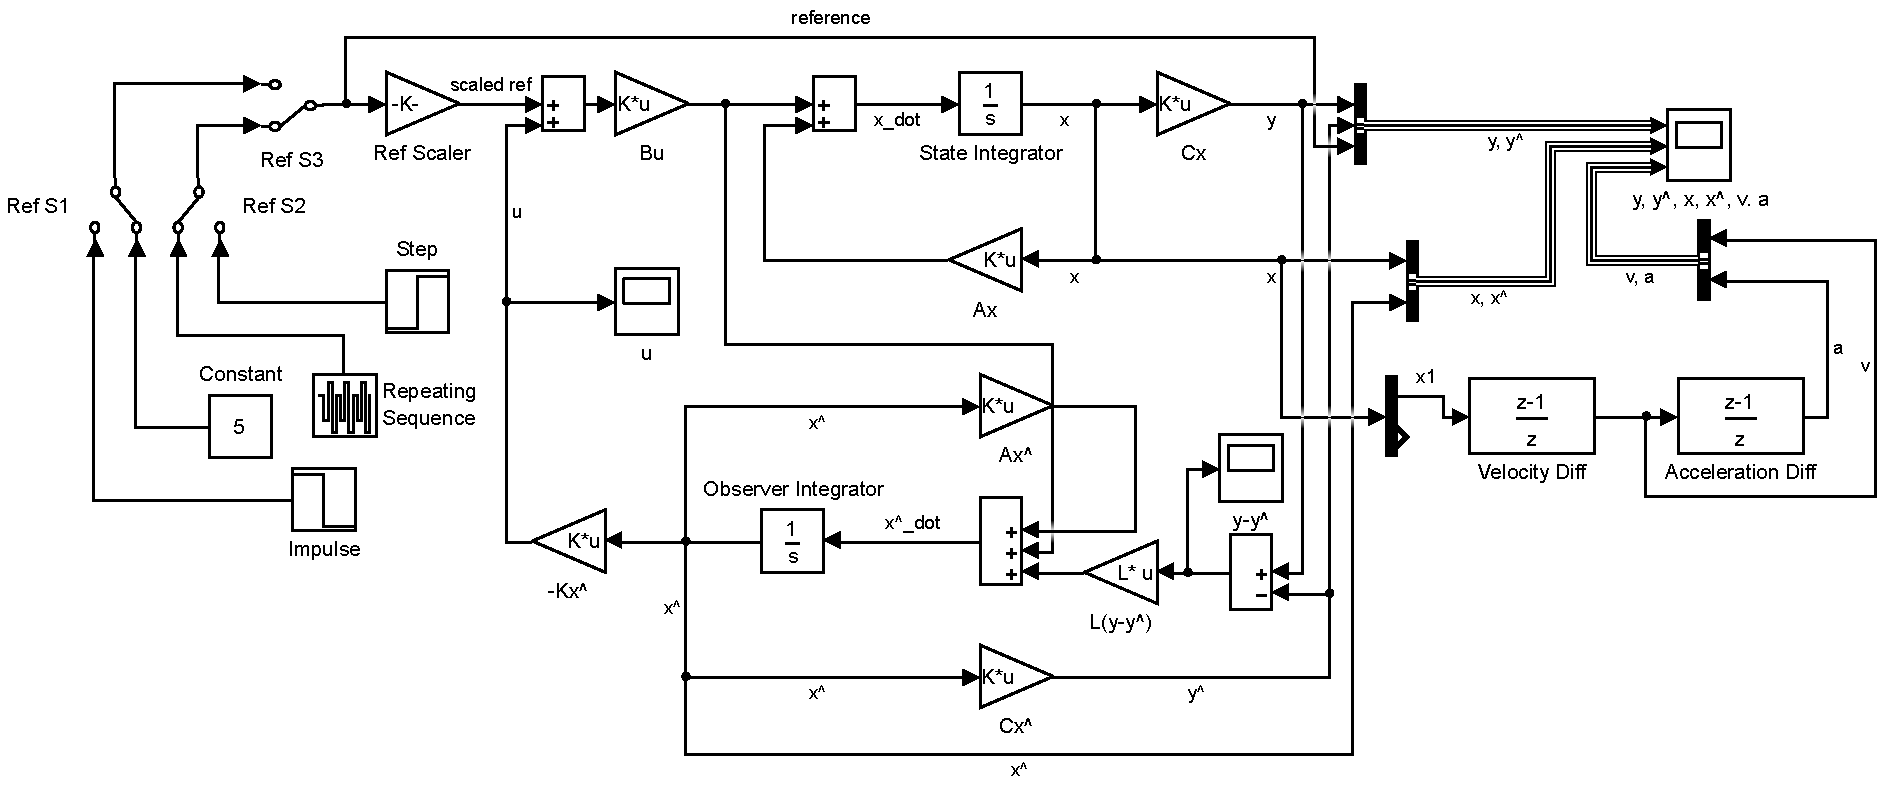
\includegraphics[angle=90, height=1.2\textheight]{resources/model.pdf}
    	\caption{The model used to simulate the observer and controller.}
    	\label{fig:simulink-model}
\end{figure}
\begin{equation}
K=
\begin{bmatrix}
  -0.064057 & -0.020791
 \end{bmatrix}
\end{equation}
And the resulting A matrix. $A’=A-KB$
\begin{equation}
A’=
\begin{bmatrix}
   -1.5405& 0.50000\\
   -0.050981 &  -1.2212
 \end{bmatrix}
\end{equation}
This clearly is no longer in observability canonical form.
\end{document}
